\documentclass[11pt, fleqn]{article}

\usepackage{amsmath}
\usepackage{amssymb}
\usepackage{amsthm}
\usepackage{mathtools}
\usepackage{hyperref}
\usepackage{ulem}
\usepackage{enumitem}
\usepackage[left=0.75in, right=0.75in, bottom=0.75in]{geometry}
% \usepackage{float}
\usepackage{floatrow}
\usepackage{graphicx}
\usepackage[export]{adjustbox}

\usepackage{sectsty}
\sectionfont{\centering}

\usepackage[perpage]{footmisc}

\usepackage{fancyhdr}
\pagestyle{fancy}
\fancyhf{}
\lhead{190100044 \& 190100055}
\rhead{CS 215: Assignment 3}
\renewcommand{\footrulewidth}{1.0pt}
\cfoot{Page \thepage}

\setlength{\parindent}{0em}
\renewcommand{\arraystretch}{2}%

\title{Assignment 3: CS 215}
\author{
\begin{tabular}{|c|c|}
     \hline
     Devansh Jain & Harshit Varma \\
     \hline
     190100044 & 190100055 \\
     \hline
\end{tabular}
}
\date{September 27, 2020}

\begin{document}

\maketitle
\tableofcontents
\thispagestyle{empty}
\setcounter{page}{0}

\renewcommand{\arraystretch}{1}

\newpage
\section*{Question 1}
\addcontentsline{toc}{section}{Question 1}
\setcounter{equation}{0}
\setcounter{figure}{0}
\subsection*{(a)}
$X_1$ denotes the number of times you have to pick a book to pick $1$ distinct color. \\ 
\boxed{X_1 = 1} (since any book you pick at the start will increment the total number of distinct books by $1$) \\

When books with $i-1$ distinct types of colors have been collected, the probability of picking a book with a different color (i.e. different from the previous $i-1$ colors) is \\
\boxed{p_i = \frac{n-(i-1)}{n} = \frac{n-i+1}{n}} \hspace{1em} \text{(Since there are $n - (i-1)$ valid choices out of $n$ possible choices)}

\subsection*{(b)}
Let's say we required $k$ additional attempts to increment the distinct no. of books from $i-1$ to $i$.\\
This would imply that for the first $k-1$ attempts, we picked a book from $i-1$ books which were selected already, and on the $k^{th}$ attempt, we chose a book from the remaining $(n - i + 1)$ books. Thus the probability that we required $k$ attempts is:
\begin{equation*}
    \begin{split}
        P(X_i = k) = \bigg(\frac{i-1}{n}\bigg)^{k-1}\bigg(\frac{n-i+1}{n}\bigg)
    \end{split}
\end{equation*}
This is exactly the PMF for a geometric random variable with the parameter $p = \bigg(\frac{n-i+1}{n}\bigg)$
% When books with $i-1$ distinct types of colors have been collected, the number of attempts to pick a bool of different color is the random variable $X_i$. \\
% Thus, $X_i$ is a geometric random variable with parameter $p_i = \frac{n-i+1}{n}$

\subsection*{(c)}
For this subsection, $Z$ is a geometric random variable with parameter $p$. \\
Probability Mass Function is $P(Z = k) = p (1-p)^{k-1}$ where $k = 1, 2, \ldots$\\
(Note that $k$ can take any arbitrary positive integer value as you can keep picking the same book again and again arbitrary number of times)\\
We use the Moment Generating function here.
\begin{equation}
    \begin{split}
        MGF = \phi_Z(t) &= \sum_{i=1}^{\infty} e^{ti} p(1-p)^{i-1} \\
            &= (e^{t} p) \sum_{i=1}^{\infty} \bigg(e^t (1-p)\bigg)^{i-1} \\
            &= \frac{e^{t} p}{(1 - e^t(1-p))} \hspace{1em} \text{(Sum of $\infty$ terms of a geometric progression)}\\
            &= \frac{p}{e^{-t} + p - 1}
    \end{split}
\end{equation}

\begin{equation}
    \begin{split}
        & \frac{d}{dt} \phi_Z(t) = \frac{p}{(e^{-t} - 1 + p)^2} (e^{-t}) \\
        & \boxed{E(Z) = \frac{d}{dt} \phi_Z(t) \bigg\rvert_{t = 0} = \frac{1}{p}} \\
    \end{split}
\end{equation}

\begin{equation}
    \begin{split}
        & \frac{d^2}{d^2t} \phi_Z(t) = \frac{p}{(e^{-t} - 1 + p)^3} (2e^{-t}) - \frac{p}{(e^{-t} - 1 + p)^2} (e^{-t}) \\
        & E(Z^2) = \frac{d^2}{d^2t} \phi_Z(t) \bigg\rvert_{t = 0} = \frac{2 - p}{p^2} \\
        & \boxed{Var(Z) = E(Z^2) - E(Z)^2 = \frac{1 - p}{p^2}} \\
    \end{split}
\end{equation}

\subsection*{(d)}
$X^{(n)} = \sum_{i=1}^{n} X_i$ where $X_i$ is a geometric random variable with $p_i = \frac{n-i+1}{n}$.
\begin{equation}
    \begin{split}
        E(X^{(n)} &= E\bigg(\sum_{i=1}^{n} X_i\bigg) \\
            &= \sum_{i=1}^{n} E(X_i) \hspace{1em} \text{(Linearity of the Expectation)}  \\
            &= \sum_{i=1}^{n} \frac{1}{p_i} \\
            &= \sum_{i=1}^{n} \frac{n}{n-i+1} \\
       \Aboxed{E(X^{(n)}) &= n \cdot \sum_{i=1}^{n} \frac{1}{n-i+1} = n \cdot \sum_{i=1}^{n} \frac{1}{i}}
    \end{split}
\end{equation}

\subsection*{(e)}
\begin{equation}
    \begin{split}
        Var(X^{(n)}) &= Var\bigg(\sum_{i=1}^{n} X_i\bigg) \\
            &= \sum_{i=1}^{n} Var(X_i) \hspace{1em} \text{(Independence of $X_i$s)} \\
            &= \sum_{i=1}^{n} \frac{1}{p_i^2} \\
            &= \sum_{i=1}^{n} \frac{n^2}{(n-i+1)^2} \\
            &= n^2 \cdot \sum_{i=1}^{n} \frac{1}{(n-i+1)^2} \\
            &= n^2 \cdot \sum_{i=1}^{n} \frac{1}{i^2} \quad \le n^2 \cdot \frac{\pi^2}{6} \\
        \Aboxed{Var(X^{(n)}) &\le \frac{\pi^2n^2}{6}}
    \end{split}
\end{equation}

\subsection*{(f)}
\subsection*{Instructions for running the code:}
\begin{itemize}[itemsep=-0.6ex]
    \item After extracting submitted file, look for a directory named \texttt{code}
    \item Within this, the code for this question is contained in a directory named \texttt{q1}
    \item Run the file \texttt{q1.m} for plotting the graph of $E(X^{(n)})$ versus $n$.
    \item \texttt{q1.png} is the plot attached in the report.
\end{itemize}
\hrule
\begin{figure}[H]
    \centering
    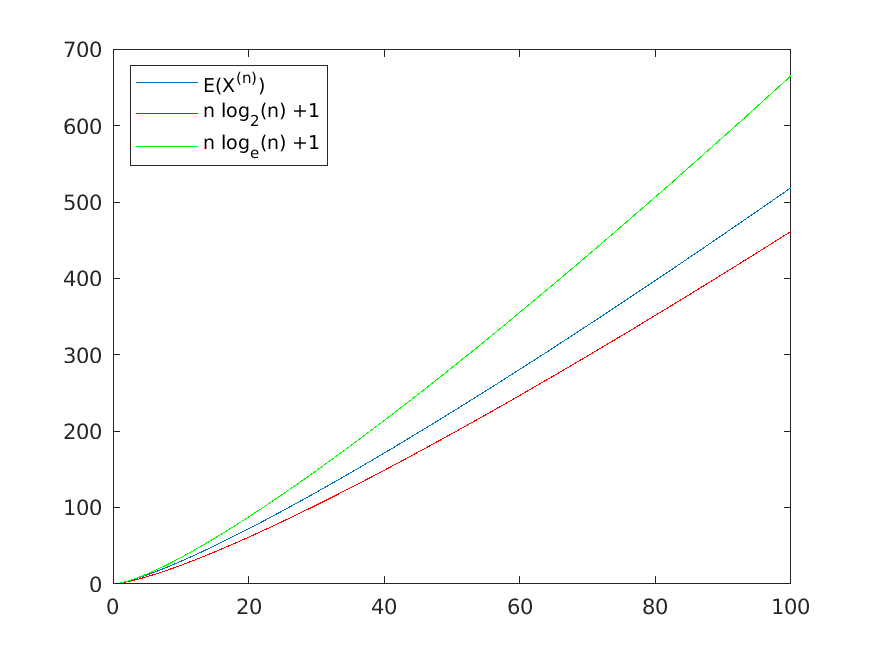
\includegraphics[width=0.8\linewidth]{q1.png}
    \caption{Plot of $E(X^{(n)})$ versus $n$ \& bounding it with $n\  log_2 (n) + 1$ \& $n\ log_e (n) + 1$}
\end{figure}
\vspace{3em}
$$\boxed{E(X^{(n)}) = \Theta(f(n))$ where $f(n) = n\ log(n)}$$


\newpage
\section*{Question 2}
\addcontentsline{toc}{section}{Question 2}
\setcounter{equation}{0}
\setcounter{figure}{0}

\subsection*{(a)}
Let $U$ be a random variable distributed as a $[0,1]$ uniform distribution, thus $\{u_i\}^{n}_{i=1}$ follows the same distribution as $U$\\
Thus,
\begin{equation}
    \label{eq:uniform}
     P(U \le u) = u 
\end{equation}

Let $V$ be a random variable such that $V = F^{-1}(U)$, thus $\{v_i\}^{n}_{i=1}$ follows the same distribution as $V$  \\
Thus CDF for $V$ is,
$$
\begin{aligned}
    P(V \le x) &= P(F^{-1}(U) \le x)\\
    &= P(U \le F(x)) \hspace{1em} \text{(Since $F$ is invertible and increasing)}\\
    &= F(x) \hspace{4.75em} \text{(Using (\ref{eq:uniform}))}
\end{aligned}
$$
Thus, $V$ is distributed as $F$.
\subsection*{(b)}
Let $U(y)$ denote the CDF for a $[0, 1]$ uniform distribution, thus $U(y) = y\  \forall y\in[0,1]$\\
Let $U_e(y) = \frac{\sum_{i=1}^n\mathbf{1}(U_i \le y)}{n} $\\
Thus, $E = \max_{0\le y\le 1} | U_e(y) - U(y) | = \max_{0\le U(y)\le 1} | U_e(y) - U(y) | $\\
Also, we have: $F_e(x) = \frac{\sum_{i=1}^n\mathbf{1}(Y_i \le x)}{n} $ and $D = \max_x | F_e(x) - F(x) |$\\
\textbf{To prove:} $P(D \ge d) = P(E \ge d), \iff P(D \le d) = P(E\le d)$\\
$$
\begin{aligned}
    %P(D \le d) &= P(\max{}_x | F_e(x) - F(x) | \le d)\\
    %&= P(| F_e(x) - F(x) | \le d) \ \forall \ x\in\mathbb{R}\\
    P(E \le d) &= P(\max{}_y | U_e(y) - U(y) | \le d)\\
    &= P(| U_e(y) - U(y) | \le d) \ \forall \ y\in [0, 1]
\end{aligned}
$$
Substituting $y = F(x)$, this can be done as both $y$ and $F(x)$ lie in $[0, 1]$ and as $F$ is continuous, it must take all values from $[0, 1]$, i.e Im($F$)=$[0, 1]$.
$$
\begin{aligned}
    P(D \le d) &= P(\max{}_x | F_e(x) - F(x) | \le d)\\
    &= P(| F_e(x) - F(x) | \le d) \ \forall \ x\in\mathbb{R}\\
    \text{ and }\\
    P(E \le d) &= P(\max{}_{F(x)} | U_e(F(x)) - U(F(x)) | \le d)\\
    &= P(| U_e(F(x)) - F(x) | \le d) \ \forall \ F(x)\in [0, 1]
\end{aligned}
$$
Now,
$$
\begin{aligned}
   U_e(F(x)) &=  \frac{\sum_{i=1}^n\mathbf{1}(U_i \le F(x))}{n}\\
   &= \frac{\sum_{i=1}^n\mathbf{1}(F^{-1}(U_i) \le x)}{n} \hspace{3em} \text{(Assuming F to be invertible\footnotemark)}\\
   &= \frac{\sum_{i=1}^n\mathbf{1}(Y_i \le x)}{n} = F_e(x) \hspace{2em} \text{(Using the results of part (a))}
\end{aligned}
$$
Thus, we get $P(E \le d) = P(| F_e(x) - F(x) | \le d) \ \forall \ F(x)\in [0, 1] = P(\max{}_{0\le F(x) \le 1} | F_e(x) - F(x) | \le d)$\\
Note that $\max{}_{0\le F(x) \le 1} | F_e(x) - F(x) | = \max{}_x | F_e(x) - F(x) | = D$, thus we get $P(E \le d) = P(D \le d)$. \\
\footnotetext{We had asked sir if can use this assumption and he had said it is ok.}

\subsection*{Practical Significance:}
% What we are essentially doing in  part (a), is ``\textbf{\textit{Inverse Transform sampling}}". \\

% For choosing $n$ random values $\{v_i\}_{i=1}^{n}$ from any distribution $F$ is equivalent of choosing $n$ random values $\{u_i\}_{i=1}^{n}$ from the uniform distribution (which is easy and the existing algorithm is highly optimized) and then applying inverse of the distribution function $F$ (apply $F^{-1}$)to random values $\{u_i\}_{i=1}^{n}$ to get $\{v_i\}_{i=1}^{n}$. \\

The random variable D measures the maximum absolute deviation of the empirical distribution (with $n$ samples) from the true distribution for an arbitrary continuous distribution $F$.\\
The random variable E measures the maximum absolute deviation of the empirical distribution (with $n$ samples) from the true distribution for the $[0, 1$] uniform distribution.\\
From the above, we can conclude that the distribution of \textit{the maximum absolute deviation of empirical distribution from true distribution} is the same (as that of an $[0, 1]$ uniform distribution with the same number of samples) irrespective of the distribution, as long as the CDF for the distribution is continuous.\\
Thus, for two arbitrary continuous distributions $F_1(x)$ and $F_2(x)$, we have:
$$
\begin{aligned}
    P(\max{}_x | F_{e_1}(x) - F_1(x) | \ge d) &= P(\max{}_{0\le y\le 1} | U_e(y) - U(y) | \ge d)\\
    P(\max{}_x | F_{e_2}(x) - F_2(x) | \ge d) &= P(\max{}_{0\le y\le 1} | U_e(y) - U(y) | \ge d)\\
    \text{Thus, }\\
    P(\max{}_x | F_{e_1}(x) - F_1(x) | \ge d) &= P(\max{}_x | F_{e_2}(x) - F_2(x) | \ge d)
\end{aligned}
$$
Thus, as a corollary of the proven result in part (b) we have shown that for any two arbitrary distributions having continuous CDFs, their maximum absolute deviation of empirical distribution from true distribution will be distributed identically.


% In part (a), we had proved that $\{v_i\}_{i=1}^{n}$ would follow the distribution F. \\
% From part (b),\\
% $P(E \le d) = P(D \le d) \implies P(\max_x | F_e(x) - F(x) | \le d) = P(\max_{0\le y\le 1} | U_e(y) - U(y) | \le d)$\\
% In other words, we can be sure with probability $P(\max_{0\le y\le 1} | U_e(y) - U(y) | \le d)$ that the absolute deviation of the empirical distribution from true distribution would be less than $d$ for all values, for any continuous distribution F.\\
% This totally justifies this method which is significantly faster and easier. \\
% This method is applied to get random values from almost all distribution including Gaussian distribution. \\
% This can actually be extended to all distribution even discrete (we had used this technique in previous homework assignments) but the proof would be more consuming. \\



\newpage
\section*{Question 3}
\addcontentsline{toc}{section}{Question 3}
\setcounter{equation}{0}
\setcounter{figure}{0}
We shall try proving a much more general result for an hyperplane in $n$ dimensional space.\\
Let the equation characterizing the hyperplane $z$ be written as $a_1x_1 + a_2x_2 + \ldots + a_nx_n + b + \varepsilon $\\
Representing in vector form, $z = \mathbf{a}^T\mathbf{x} + b + \varepsilon$ where $\mathbf{a} = [a_1 \ldots a_n]^T \in \mathbb{R}^n$, $\mathbf{x} = [x_1 \ldots x_n]^T \in \mathbb{R}^n$ and $b \in \mathbb{R}$ and $\varepsilon$ is the gaussian noise.\\
Thus, as the noise $\varepsilon \thicksim \mathcal{N}(0, \sigma^2)$, 
$ z_i \thicksim \mathcal{N}( \mathbf{a}^T\mathbf{x_i}+b, \sigma^2) $ where $i$ denotes the $i^{th}$ sample point.\\
Thus the likelihood $p(\{z_i\}_i;\mathbf{x_i}, \mathbf{a}, b)$ is given as:
\begin{equation*}
    \begin{split}
        p(\{z_i\}_i;\mathbf{x_i}, \mathbf{a}, b) = \prod_{i=1}^{N}\frac{1}{\sigma\sqrt{2\pi}} \exp{\bigg(\frac{(z_i - (\mathbf{a}^T\mathbf{x_i} + b))^2}{2\sigma^2}\bigg)}
    \end{split}
\end{equation*}
Taking the $\log$, we obtain the log likelihood:
\begin{equation}
    \label{logl}
    \begin{split}
        \boxed{\mathcal{L} = \log{p(\{z_i\}_i;\mathbf{x_i}, \mathbf{a}, b)} = -\frac{1}{{2\sigma^2}}\sum_{i=1}^{N} (z_i - (\mathbf{a}^T\mathbf{x_i} + b))^2 - N\log(\sigma\sqrt{2\pi})}
    \end{split}
\end{equation}
Next, we compute the partial derivatives of $\mathcal{L}$ w.r.t the parameters and equate them to 0.
\begin{equation*}
    \begin{split}
        \frac{\partial \mathcal{L}}{\partial \mathbf{a}} = \bigg( \frac{\partial \mathcal{L}}{\partial a_1}, \ldots, \frac{\partial \mathcal{L}}{\partial a_n} \bigg) = \mathbf{0} = (0, \dots, 0) \text{ and } \frac{\partial \mathcal{L}}{\partial b} = 0 
    \end{split}
\end{equation*}
Thus,
\begin{equation*}
    \begin{split}
        \frac{\partial \mathcal{L}}{\partial \mathbf{a}} = \mathbf{0} \Rightarrow \frac{\partial \mathcal{L}}{\partial a_j} = 0 \ \forall \ j = 1,\ldots,n
    \end{split}
\end{equation*}
Note that $i = 1,\ldots,N$ and $j = 1,\ldots,n$\\
\begin{equation*}
    \begin{split}
        \frac{\partial \mathcal{L}}{\partial a_j} = \frac{1}{{\sigma^2}}\sum_{i=1}^{N} (z_i - (\mathbf{a}^T\mathbf{x_i} + b))\frac{\partial (\mathbf{a}^T\mathbf{x_i})}{\partial a_j} = \frac{1}{{\sigma^2}}\sum_{i=1}^{N} (z_i - (\mathbf{a}^T\mathbf{x_i} + b))x_{ij} = 0
    \end{split}
\end{equation*}
and,
\begin{equation*}
    \begin{split}
        \frac{\partial \mathcal{L}}{\partial b} = \frac{1}{{\sigma^2}}\sum_{i=1}^{N} (z_i - (\mathbf{a}^T\mathbf{x_i} + b)) = 0
    \end{split}
\end{equation*}
Thus, we get:
\begin{equation}
    \label{set1}
    \begin{split}
        \boxed{\sum_{i=1}^{N} x_{ij}(\mathbf{a}^T\mathbf{x_i}) + b\sum_{i=1}^{N}(x_{ij}) = \sum_{i=1}^{N} (z_ix_{ij}) \  \ \forall \ j = 1,\ldots,n}
    \end{split}
\end{equation}
and,
\begin{equation}
    \label{set2}
    \begin{split}
        \boxed{\sum_{i=1}^{N}\big((\mathbf{a}^T\mathbf{x_i}) + b\cdot1 \big) = \sum_{i=1}^{N} z_i}
    \end{split}
\end{equation}
Thus we have $n+1$ equations for $n+1$ variables.

We can condense \eqref{set1} and \eqref{set2} into a single equation in the form of matrices and vectors as:
\begin{equation}
    \sum_{i=1}^{N}
    \begin{bmatrix}
        z_i x_{i1} \\
        z_i x_{i2} \\
        \vdots \\
        z_i x_{in} \\
        z_i \\
    \end{bmatrix}
    =
    \sum_{i=1}^{N}
    \begin{bmatrix}
        x_i \\
        x_2 \\
        \vdots \\
        x_n \\
        1 \\
    \end{bmatrix}
    \begin{bmatrix}
        x_i & x_2 & \cdots & x_n & 1 \\
    \end{bmatrix}
    \begin{bmatrix}
        a_i \\
        a_2 \\
        \vdots \\
        a_n \\
        b \\
    \end{bmatrix}
\end{equation}

\subsection*{(a)}
Given $z = ax + by +c$. \\
As the noise $\varepsilon \thicksim \mathcal{N}(0, \sigma^2)$, we have $ z_i \thicksim \mathcal{N}(a x_i + b y_i + c, \sigma^2) $ where $i \in (0, N)$ denotes the $i^{th}$ sample point. \\
Thus the likelihood $p(\{z_i\}_i; \{x_i\}, a, b, c)$ is given as:
\begin{equation*}
    \begin{split}
        p(\{z_i\}; \{x_i\}, \{y_i\}, a, b, c) = \prod_{i=1}^{N}\frac{1}{\sigma\sqrt{2\pi}} \exp{\bigg(\frac{(z_i - (ax_i + by_i + c))^2}{2\sigma^2}\bigg)}
    \end{split}
\end{equation*}
Taking the $\log$, we obtain the log likelihood:
\begin{equation}
    \label{logl1}
    \begin{split}
        \boxed{\mathcal{L} = \log{p(\{z_i\}; \{x_i\}, \{y_i\}, a, b, c)} = - n\log(\sigma\sqrt{2\pi}) -\frac{1}{{2\sigma^2}}\sum_{i=1}^{N} (z_i - (ax_i + by_i + c))^2 }
    \end{split}
\end{equation}
Next, we compute the partial derivatives of $\mathcal{L}$ w.r.t the parameters (a, b, c) and equate them to 0.
\begin{equation*}
    \begin{split}
        \frac{\partial \mathcal{L}}{\partial a} &= \frac{1}{{\sigma^2}}\sum_{i=1}^{N} (z_i - (ax_i + by_i + c)) x_i = 0 \Longrightarrow \sum_{i=1}^{N} z_ix_i = \sum_{i=1}^{N} (ax_i + by_i + c)) x_i \\
        \frac{\partial \mathcal{L}}{\partial b} &= \frac{1}{{\sigma^2}}\sum_{i=1}^{N} (z_i - (ax_i + by_i + c)) y_i = 0 \Longrightarrow \sum_{i=1}^{N} z_iy_i = \sum_{i=1}^{N} (ax_i + by_i + c)) y_i \\
        \frac{\partial \mathcal{L}}{\partial c} &= \frac{1}{{\sigma^2}}\sum_{i=1}^{N} (z_i - (ax_i + by_i + c)) = 0 \Longrightarrow \sum_{i=1}^{N} z_i = \sum_{i=1}^{N} (ax_i + by_i + c)) \\
    \end{split}
\end{equation*}
Matrix and vector form:
\begin{equation}
    \sum_{i=1}^{N}
    \begin{bmatrix}
        z_i x_i \\
        z_i y_i \\
        z_i \\
    \end{bmatrix}
    =
    \sum_{i=1}^{N}
    \begin{bmatrix}
        x_i^2 & x_i y_i & x_i \\
        x_i y_i & y_i^2 & y_i \\
        x_i & y_i & 1 \\
    \end{bmatrix}
    \begin{bmatrix}
        a \\
        b \\
        c \\
    \end{bmatrix}
    =
    \sum_{i=1}^{N}
    \begin{bmatrix}
        x_i \\
        y_i \\
        1 \\
    \end{bmatrix}
    \begin{bmatrix}
        x_i & y_i & 1 \\
    \end{bmatrix}
    \begin{bmatrix}
        a \\
        b \\
        c \\
    \end{bmatrix}
\end{equation}

\subsection*{(b)}
Given $z = f(x,y) = a_1 x^2 + a_2 y^2 + a_3 xy + a_4 x + a_5 y + a_6$. \\
As the noise $\varepsilon \thicksim \mathcal{N}(0, \sigma^2)$, we have $ z_i \thicksim \mathcal{N}(f(x_i, y_i), \sigma^2) $ where $i \in (0, N)$ denotes the $i^{th}$ sample point. \\
Thus the likelihood $p(\{z_i\}_i; \{x_i\}, a_1, a_2, a_3, a_4, a_5, a_6)$ is given as:
\begin{equation*}
    \begin{split}
        p(\{z_i\}; \{x_i\}, \{y_i\}, a_1, a_2, a_3, a_4, a_5, a_6c) = \prod_{i=1}^{N}\frac{1}{\sigma\sqrt{2\pi}} \exp{\bigg(\frac{(z_i - (f(x_i,y_i))^2}{2\sigma^2}\bigg)}
    \end{split}
\end{equation*}
Taking the $\log$, we obtain the log likelihood:
\begin{equation}
    \label{logl2}
    \begin{split}
        \boxed{\mathcal{L} = \log{p(\{z_i\}; \{x_i\}, \{y_i\}, a_1, a_2, a_3, a_4, a_5, a_6)} = - n\log(\sigma\sqrt{2\pi}) -\frac{1}{{2\sigma^2}}\sum_{i=1}^{N} (z_i - (f(x_i,y_i))^2 }
    \end{split}
\end{equation}
Next, we compute the partial derivatives of $\mathcal{L}$ w.r.t the parameters and equate them to 0.
\begin{equation*}
    \begin{split}
        \frac{\partial \mathcal{L}}{\partial a_1} &= \frac{1}{{\sigma^2}}\sum_{i=1}^{N} (z_i - f(x_i,y_i)) x_i^2 = 0 \Longrightarrow \sum_{i=1}^{N} z_i x_i^2 = \sum_{i=1}^{N} (a_1 x_i^2 + a_2 y_i^2 + a_3 x_iy_i + a_4 x_i + a_5 y_i + a_6) x_i^2\\
        \frac{\partial \mathcal{L}}{\partial a_2} &= \frac{1}{{\sigma^2}}\sum_{i=1}^{N} (z_i - f(x_i,y_i)) y_i^2 = 0 \Longrightarrow \sum_{i=1}^{N} z_i y_i^2= \sum_{i=1}^{N} (a_1 x_i^2 + a_2 y_i^2 + a_3 x_iy_i + a_4 x_i + a_5 y_i + a_6) y_i^2\\
        \frac{\partial \mathcal{L}}{\partial a_3} &= \frac{1}{{\sigma^2}}\sum_{i=1}^{N} (z_i - f(x_i,y_i)) x_iy_i = 0 \Longrightarrow \sum_{i=1}^{N} z_i x_iy_i= \sum_{i=1}^{N} (a_1 x_i^2 + a_2 y_i^2 + a_3 x_iy_i + a_4 x_i + a_5 y_i + a_6) x_iy_i\\
        \frac{\partial \mathcal{L}}{\partial a_4} &= \frac{1}{{\sigma^2}}\sum_{i=1}^{N} (z_i - f(x_i,y_i)) x_i = 0 \Longrightarrow \sum_{i=1}^{N} z_i x_i= \sum_{i=1}^{N} (a_1 x_i^2 + a_2 y_i^2 + a_3 x_iy_i + a_4 x_i + a_5 y_i + a_6) x_i\\
        \frac{\partial \mathcal{L}}{\partial a_5} &= \frac{1}{{\sigma^2}}\sum_{i=1}^{N} (z_i - f(x_i,y_i)) y_i = 0 \Longrightarrow \sum_{i=1}^{N} z_i y_i= \sum_{i=1}^{N} (a_1 x_i^2 + a_2 y_i^2 + a_3 x_iy_i + a_4 x_i + a_5 y_i + a_6) y_i\\
        \frac{\partial \mathcal{L}}{\partial a_6} &= \frac{1}{{\sigma^2}}\sum_{i=1}^{N} (z_i - f(x_i,y_i)) = 0 \Longrightarrow \sum_{i=1}^{N} z_i = \sum_{i=1}^{N} (a_1 x_i^2 + a_2 y_i^2 + a_3 x_iy_i + a_4 x_i + a_5 y_i + a_6)\\
    \end{split}
\end{equation*}
Matrix and vector form:
\begin{equation}
    \sum_{i=1}^{N}
    \begin{bmatrix}
        z_i x_i^2 \\
        z_i y_i^2 \\
        z_i x_i y_i \\
        z_i x_i \\
        z_i y_i \\
        z_i \\
    \end{bmatrix}
    =
    \sum_{i=1}^{N}
    \begin{bmatrix}
        x_i^2 \\
        y_i^2 \\
        x_i y_i \\
        x_i \\
        y_i \\
        1 \\
    \end{bmatrix}
    \begin{bmatrix}
        x_i^2 & y_i^2 & x_i y_i & x_i & y_i & 1 \\
    \end{bmatrix}
    \begin{bmatrix}
        a_1 \\
        a_2 \\
        a_3 \\
        a_4 \\
        a_5 \\
        a_6 \\
    \end{bmatrix}
\end{equation}

\subsection*{(c)}
\subsection*{Instructions for running the code:}
\begin{itemize}
    \item After extracting submitted file, look for a directory named \texttt{code}.
    \item Within this, the code for this question is contained in a directory named \texttt{q3}
    \item Run the file \texttt{q3.m} for predicting the equation of the plane and noise variance.
\end{itemize}
On running the code with \texttt{XYZ.txt} as the input file, \\
Output:
\begin{figure}[H]
    \vspace{-1em}
    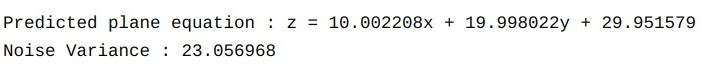
\includegraphics[width=0.8\linewidth, left]{output.jpeg}
\end{figure}
\vspace{-1em}
Thus, the predicted equation of plane is \boxed{$z = 10x + 20y + 30$} and noise variance is \boxed{23}.


\newpage
\section*{Question 4}
\addcontentsline{toc}{section}{Question 4}
\setcounter{equation}{0}
\setcounter{figure}{0}
\subsection*{Instructions for running the code:}
\begin{itemize}[itemsep=-0.6ex]
    \item After extracting submitted file, look for a directory named \texttt{code}
    \item Within this, the code for this question is contained in a directory named \texttt{q4}
    \item Run the file \texttt{q4.m}, this generates the 4 required plots and prints out the values asked for
    \item Note: \texttt{q4\_v\_equal\_t.m} generates the plots for part (e)
\end{itemize}
\hrule
\vspace{15pt}
There are $N\ (=1000)$ samples in our dataset ($X$). \\
There are $n\ (=750)$ samples in our training set. \\
There are $m\ (=250)$ samples in our validation set. \\
Let the training set $T$ be given by $T = \{t_i\}_{i=1}^n$ \\
Let the validation set $V$ be given by $V = \{v_j\}_{j=1}^m$ \\
Also, $T\cap V = \phi$ and $T \cup V = X$ \\
Thus, we have the Gaussian kernel estimator as: \\
$$
\hat p_n(x;\sigma) = \frac{1}{n\sigma\sqrt{2\pi}} \sum_{i=1}^{n}\exp\bigg(\frac{-(x - t_i)^2}{2\sigma^2} \bigg)
$$
\subsection*{(b)}
Therefore, the joint likelihood of the samples in $V$, assuming $\{v_j\}_{j=1}^{m}$ to be independent, is:
$$
\begin{aligned}
    f(\{v_j\}_{j=1}^{m}; \sigma) &= \prod_{j=1}^m \hat p_n(v_j;\sigma)\\
    &= \Aboxed{\bigg(\frac{1}{n\sigma\sqrt{2\pi}}\bigg)^m\cdot \prod_{j=1}^m\Bigg( \sum_{i=1}^{n}\exp\bigg(\frac{-(v_j - t_i)^2}{2\sigma^2} \bigg) \Bigg)}
\end{aligned}
$$
The log-likelihood is given by:
$$
\begin{aligned}
    \log f(\{v_j\}_{j=1}^{m}; \sigma) &= \sum_{j=1}^m \log (\hat p_n(v_j;\sigma))\\
    &= \Aboxed{\sum_{j=1}^m \log \bigg(\sum_{i=1}^{n}\exp\bigg(\frac{-(v_j - t_i)^2}{2\sigma^2} \bigg)\bigg) - m\log(n\sigma\sqrt{2\pi})}
\end{aligned}
$$
\subsection*{(c)}
\begin{figure}[H]
    \centering
    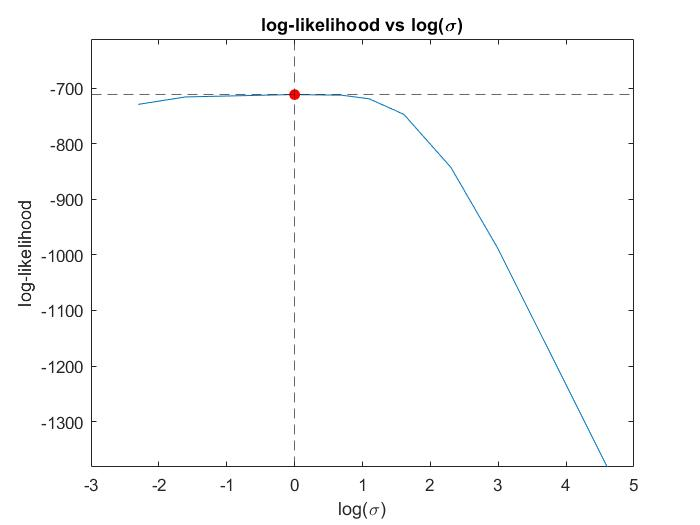
\includegraphics[scale=0.4]{q4ci.jpg}
    \caption{$\log f(\{v_j\}_{j=1}^{m}; \sigma)$ vs $\log(\sigma)$}
    \label{fig:q4ci}
\end{figure}

$\boxed{\sigma = 1 }$ yields the maximum value of the log-likelihood.

\begin{figure}[H]
    \centering
    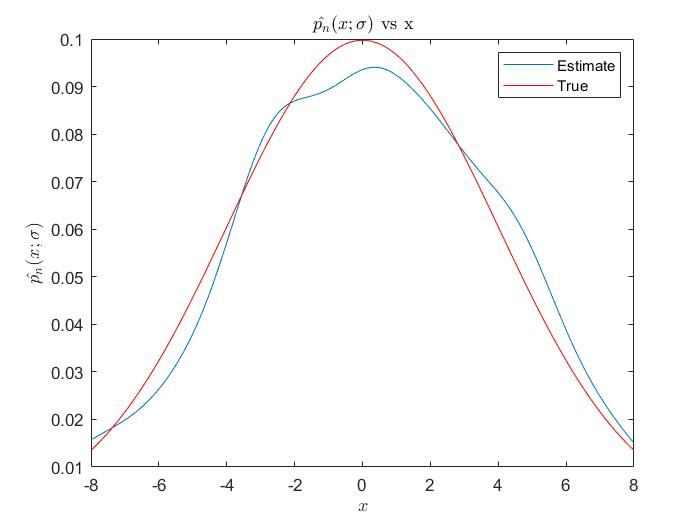
\includegraphics[scale=0.4]{q4cii.jpg}
    \caption{True PDF overlaid on the estimated PDF}
    \label{fig:q4cii}
\end{figure}
\newpage

\subsection*{(d)}
\begin{figure}[H]
    \centering
    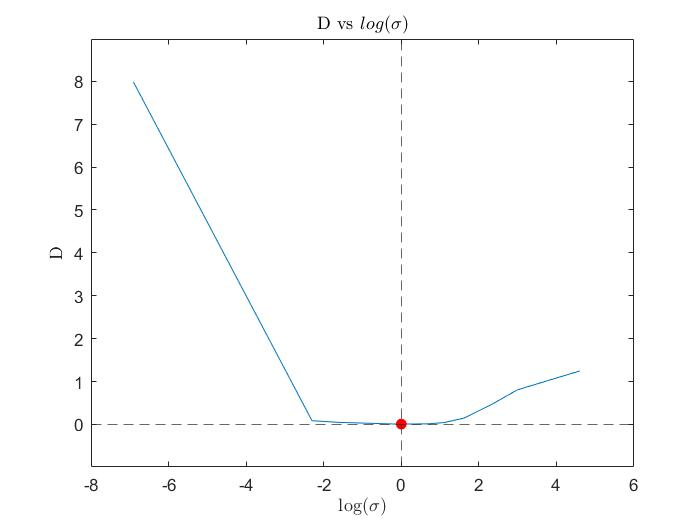
\includegraphics[scale=0.41]{q4di.jpg}
    \caption{D vs $\log(\sigma)$}
    \label{fig:q4di}
\end{figure}

\begin{figure}[H]
    \centering
    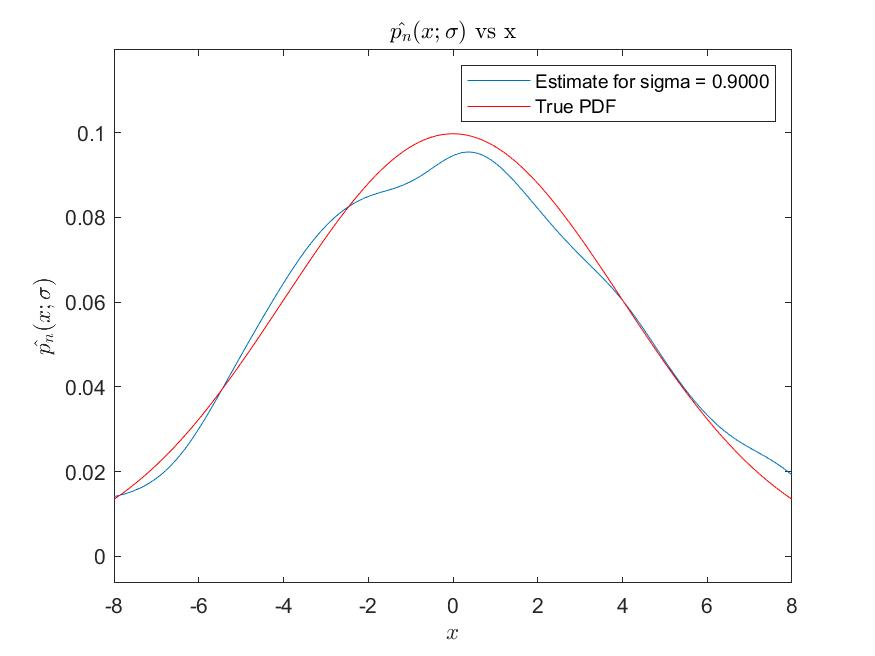
\includegraphics[scale=0.41]{q4dii.jpg}
    \caption{True PDF overlaid on the estimated PDF}
    \label{fig:q4dii}
\end{figure}
\newpage

\begin{verbatim}
    Best sigma that minimizes D:  0.9000
    The value of D at this sigma(= 0.9000) is:  0.0048
    D value for the sigma parameter that yielded the best LL:  0.0049
\end{verbatim}

\subsection*{(e)}
Let $V = T$, thus, $m = n$\\
The new log-likelihood is given by:
$$
\begin{aligned}
    \mathcal{L} = \log f(\{t_j\}_{j=1}^{n}; \sigma) &= \sum_{j=1}^n \log \bigg(\sum_{i=1}^{n}\exp\bigg(\frac{-(t_j - t_i)^2}{2\sigma^2} \bigg)\bigg) - n\log(n\sigma\sqrt{2\pi})
\end{aligned}
$$
$$
\begin{aligned}
    \frac{\partial\mathcal{L}}{d\sigma} = -\frac{n}{\sigma} + \sum_{j=1}^n \left( \frac{1}{\bigg(\sum_{i=1}^{n}\exp\frac{-(t_j - t_i)^2}{2\sigma^2}\bigg)}\cdot \sum_{i=1}^{n}\Bigg(\frac{(t_j - t_i)}{\sigma^3} \exp\bigg(\frac{-(t_j - t_i)^2}{2\sigma^2}\bigg) \Bigg) \right) < 0
\end{aligned}
$$

The log-likelihood comes out to be strictly decreasing as the second term evaluates to $0$ (due to anti-symmetry), thus in the cross-validation procedure, the smallest value of $\sigma$ will be selected as this will maximize the log-likelihood. (Thus, we get wrong $\sigma$ value from the cross-validation procedure)\\
This corresponds to the \textbf{\textit{undersmoothening}} case.\\
As $\hat p_n(x;\sigma)$ is constituted by $n$ smaller gaussians (centered at $t_i$s) added together, a small value of $\sigma$ (which in this case also happens to be the variance of the individual gaussians) will lead to each constituent gaussian having a sharper peak at there respective centres ($t_i$s), thus $\hat p_n(x;\sigma)$ will have sharp peaks at the $t_i$ values (can be seen in the plot obtained by taking the $\sigma$ returned by the cross-validation procedure - Fig. \ref{fig:q4d_extra1})\\
Therefore, if we used this $\hat p_n(x;\sigma)$, cross-validated as well as trained on $T$, our results won't generalize well on an unseen sample.


\begin{figure}[H]
    \centering
    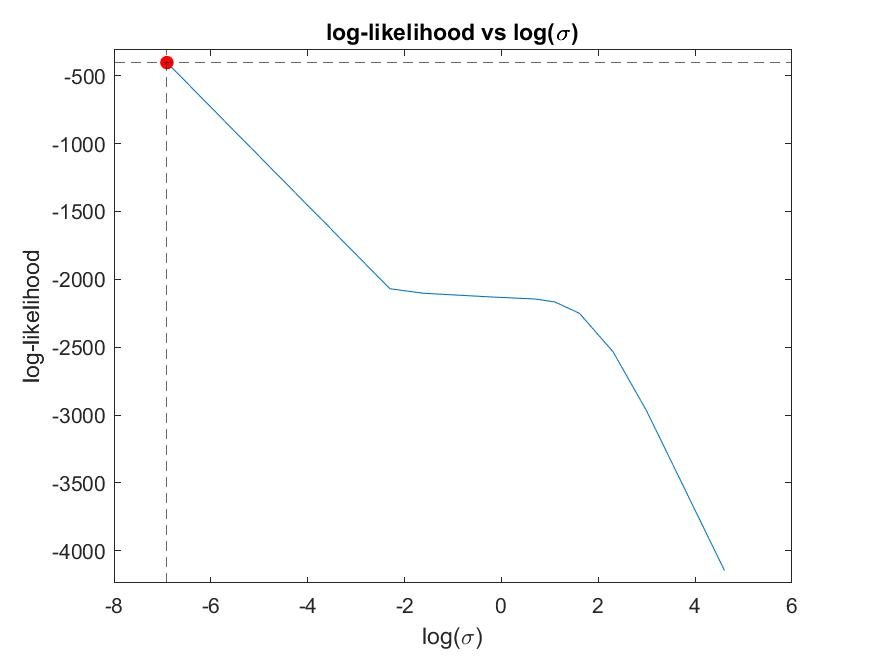
\includegraphics[scale=0.4]{q4d_extra2.jpg}
    \caption{$\log f(\{v_j\}_{j=1}^{m}; \sigma)$ vs $\log(\sigma)$ for $V=T$}
    \label{fig:q4d_extra2}
\end{figure}

\begin{figure}[H]
    \centering
    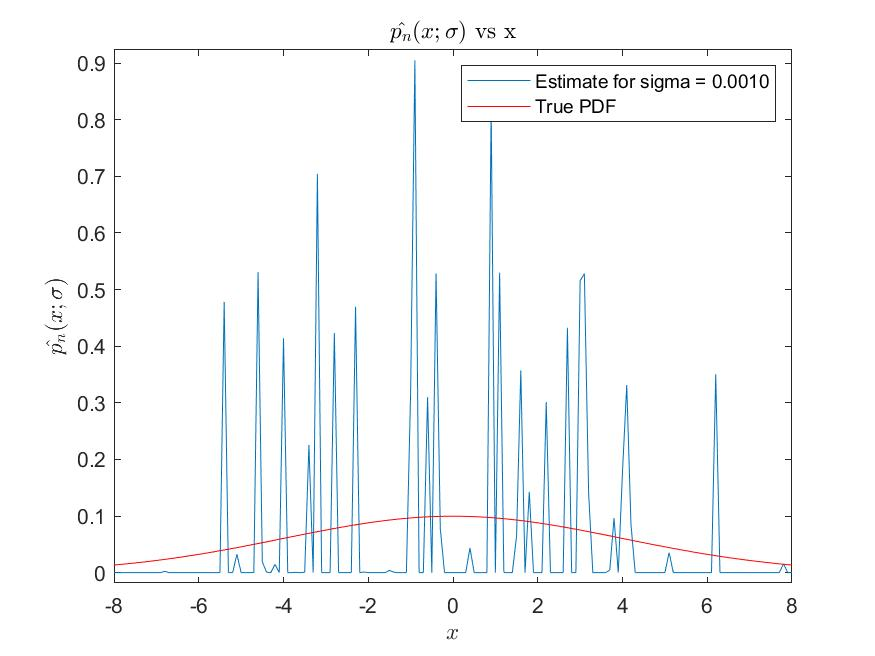
\includegraphics[scale=0.4]{q4d_extra1.jpg}
    \caption{True PDF overlaid on the estimated PDF with $V=T$}
    \label{fig:q4d_extra1}
\end{figure}

\end{document}
